\documentclass[11pt, oneside]{article}   	% use "amsart" instead of "article" for AMSLaTeX format
\usepackage{geometry}
\usepackage{amsmath}              		% See geometry.pdf to learn the layout options. There are lots.
\geometry{letterpaper}                   		% ... or a4paper or a5paper or ... 
%\geometry{landscape}                		% Activate for for rotated page geometry
%\usepackage[parfill]{parskip}    		% Activate to begin paragraphs with an empty line rather than an indent
\usepackage{graphicx}				% Use pdf, png, jpg, or eps§ with pdflatex; use eps in DVI mode
								% TeX will automatically convert eps --> pdf in pdflatex		
\usepackage{amssymb}
\usepackage{mcode}

\title{CS 6220 - Assignment 4}
\author{Ally Warner}
%\date{}							% Activate to display a given date or no date

\begin{document}
\maketitle

\begin{enumerate}

\item Consider the boundary value ODE
\[
-(au')' = q, \quad 0 < x < 1,
\]
\[
u(0) = 0, \quad u'(1) = 0,
\]
where $a(x) > 0$ and $q(x)$ are known, smooth functions. It is well known (recall Section 3.1.3) that $u$ also minimizes,
\[
T = \int_0^1 [a(u')^2 - 2uq]dx
\]
over all functions with bounded first derivatives that satisfy the essential BC $u(0) = 0$. Consider next discretizing the integral on a nonuniform mesh,
\[
0 = x_0 < x_1 < \dots < x_J = 1,
\]
as in Exercises 2 and 3.

\begin{enumerate}

\item Show that, applying the midpoint rule for the first term and the trapezoidal rule for the second term in $T$ for each subinterval, one obtains the problem of minimizing
\[
T_h = \sum_{i=0}^{J-1} a(x_{i + \frac{1}{2}}) \frac{(v_{i+1} - v_i)^2}{h_i} - h_i(q(x_i)v_i + q(x_{i+1}) v_{i+1})
\]
with $v_0 = 0$. Thus, $T_h(u) = T(u) + \mathcal{O}(h^2)$, where $h = \max_i h_i$.

\vspace{5mm}

By separating the integral, applying the midpoint rule to the first term and the trapezoidal rule for the second term and evaluating the second integral, we get the following,
\[
T = \int_0^1 a(x_{i+\frac{1}{2}}) \left(\frac{v_{i+1} - v_i}{h_i}\right)^2 dx - 2\left(\frac{h_i}{2} (v_i q(x_i) + v_{i+1} q(x_{i+1}))\right).
\]
Since we are evaluating at every subinterval and since we are finding area under a curve (we are evaluating an integral), we need to include the width with the area that we already have the height of which is $h_i$. So evaluating the first integral gives the following,
\[
T = \sum^{J-1}_{i = 0} h_i a(x_{i+\frac{1}{2}}) \left(\frac{v_{i+1} - v_i}{h_i}\right)^2 - h_i (v_i q(x_i) + v_{i+1} q(x_{i+1}))
\]
and gives us the end result of
\[
T_h = \sum^{J-1}_{i = 0} a(x_{i+\frac{1}{2}}) \frac{(v_{i+1} - v_i)^2}{h_i} - h_i (v_i q(x_i) + v_{i+1} q(x_{i+1})).
\] 

\item Obtain the necessary conditions
\[
a(x_{j+\frac{1}{2}}) \frac{v_j - v_{j+1}}{h_j} + a(x_{j - \frac{1}{2}}) \frac{v_j - v_{j-1}}{h_{j-1}} = \frac{h_j + h_{j-1}}{2} q(x_j)
\]
for $j = 1, \dots, J$, where we set $v_{J+1} = v_J$.

\vspace{5mm}

Since we are minimizing the equation in part a, we will take the derivative of $T_h$ and equal it to zero. Since $T_h$ involves a sum, we will need to look at different instances of the index $i$. 

First let $i = j-1$.
\[
T_h = a(x_{j-\frac{1}{2}}) \frac{(v_j - v_{j-1})^2}{h_{j-1}} - h_{j-1}(v_{j-1} q(x_{j-1}) + v_j q(x_j))
\]
\[
\frac{dT_h}{d v_j} = a(x_{j - \frac{1}{2}}) 2 \frac{v_j - v_{j-1}}{h_{j-1}} - h_{j-1} q(x_j)
\]
Then let $i = j$.
\[
T_h = a(x_{j+\frac{1}{2}}) \frac{(v_{j+1} - v_j)^2}{h_j} - h_j (v_j q(x_j) + v_{j+1} q(x_{j+1}))
\]
\[
\frac{dT_h}{d v_j} = a(x+\frac{1}{2}) (-2)\frac{v_{j+1} - v_j}{h_j} - h_j q(x_j)
\]
Adding these derivate terms together and setting them equal to zero yields the desired equation.
\[
a(x_{j+\frac{1}{2}}) \frac{v_j - v_{j+1}}{h_j} + a(x_{j - \frac{1}{2}}) \frac{v_j - v_{j-1}}{h_{j-1}} = \frac{h_j + h_{j-1}}{2} q(x_j)
\]

\item Show that upon writing the above as a linear system of equations $A$\textbf{v} = \textbf{q}, the matrix $A$ is tridiagonal, symmetric, and positive definite despite the arbitrary nonuniformity of the mesh.

\vspace{5mm}

From the equation in part b, we group together the terms corresponding to $v_{i-1}$, $v_i$, and $v_{i+1}$ and obtain the following,
\[
\frac{h_i + h_{i-1}}{2} q(x_i) = \left(\frac{-a(x_{i-\frac{1}{2}})}{h_{i-1}}\right) v_{i-1} + \left( \frac{a(x_{i+\frac{1}{2}})}{h_i} + \frac{a(x_{i-\frac{1}{2}})}{h_{i-1}} \right) v_i + \left(\frac{-a(x_{i+\frac{1}{2}})}{h_i}\right) v_{i+1}
\]
which gives the coefficients to build the matrix $A$. We know that $A$ is tridiagonal because it only has three terms that shift in every row. We can show that it is symmetric by checking the $i-1$ and $i+1$ rows and comparing terms. 

Row $i-1$:
\[
\frac{h_{i+1} + h_{i}}{2} q(x_{i+1}) = \left(\frac{-a(x_{i-\frac{3}{2}})}{h_{i-2}}\right) v_{i-2} + \left( \frac{a(x_{i-\frac{1}{2}})}{h_{i-1}} + \frac{a(x_{i-\frac{3}{2}})}{h_{i-2}} \right) v_{i-1} + \left(\frac{-a(x_{i-\frac{1}{2}})}{h_{i-1}}\right) v_{i}
\]

Row $i+1$:
\[
\frac{h_{i-1} + h_{i-2}}{2} q(x_{i-1}) = \left(\frac{-a(x_{i+\frac{1}{2}})}{h_{i}}\right) v_{i} + \left( \frac{a(x_{i+\frac{3}{2}})}{h_{i+1}} + \frac{a(x_{i+\frac{1}{2}})}{h_{i}} \right) v_{i+1} + \left(\frac{-a(x_{i+\frac{3}{2}})}{h_{i+1}}\right) v_{i+2}
\]
Since the $i$th$-1$ row has the same coefficient for $v_i$ as the $v_{i-1}$ term in the $i$th row, and the $i$th$+1$ row has the same coefficient for $v_i$ as the $v_{i+1}$ term in the $i$th row, $A$ is symmetric. This can be seen in the matrix representation of these rows below.
\[
\begin{bmatrix}
\frac{-a(x_{i-\frac{3}{2}})}{h_{i-2}} & \frac{a(x_{i-\frac{1}{2}})}{h_{i-1}} + \frac{a(x_{i-\frac{3}{2}})}{h_{i-2}} & \frac{-a(x_{i-\frac{1}{2}})}{h_{i-1}} & &\\
 & \frac{-a(x_{i-\frac{1}{2}})}{h_{i-1}} &  \frac{a(x_{i+\frac{1}{2}})}{h_i} + \frac{a(x_{i-\frac{1}{2}})}{h_{i-1}} & \frac{-a(x_{i+\frac{1}{2}})}{h_i} &\\
& & \frac{-a(x_{i+\frac{1}{2}})}{h_i} & \frac{a(x_{i+\frac{3}{2}})}{h_{i+1}} + \frac{a(x_{i+\frac{1}{2}})}{h_{i}} & \frac{-a(x_{i+\frac{3}{2}})}{h_{i+1}}\\
\end{bmatrix}
\]

To test if $A$ is positive definite, we will use the following theorem.  A symmetric matrix is positive definite if each diagonal entry is equal to the sum of the absolute values of all other entries in the row/column in which it appears with the exception of at least one row where it is greater. This is true for A due to our boundary conditions which makes the first entry in the first row 1 followed by zeros. We can also see that the rest of the rows are equal.

\end{enumerate}

\item Convince yourself by running a computational example that the solution \textbf{v} is a second order accurate despite what Exercise 3 may suggest. Then try to prove it.

For your computational experiments, take $a(x) = 1.0 + e^z$ and $q(x) = \pi^2 \sin(\pi x)$. Compare using a uniform mesh with an element spacings of $\frac{1}{20}, \frac{1}{40}, \frac{1}{80}$, and $\frac{1}{160}$ and a set of four non-uniform meshes generated by golden ratio subdivision. To generate your non-uniform meshes, your base mesh should be a uniform mesh with spacing of $\frac{1}{20}$. Let a depth-1 subdivision be the splitting of these 20 elements into 40 elements using the golden ratio partitioning on each element. Recursively design your four non-uniform meshes from depth-1 to depth-4. Comment on your results.

\vspace{5mm}

The following figure shows the solution \textbf{v} on a uniform mesh at different mesh refinements.

\vspace{2mm}

\centerline {\frame{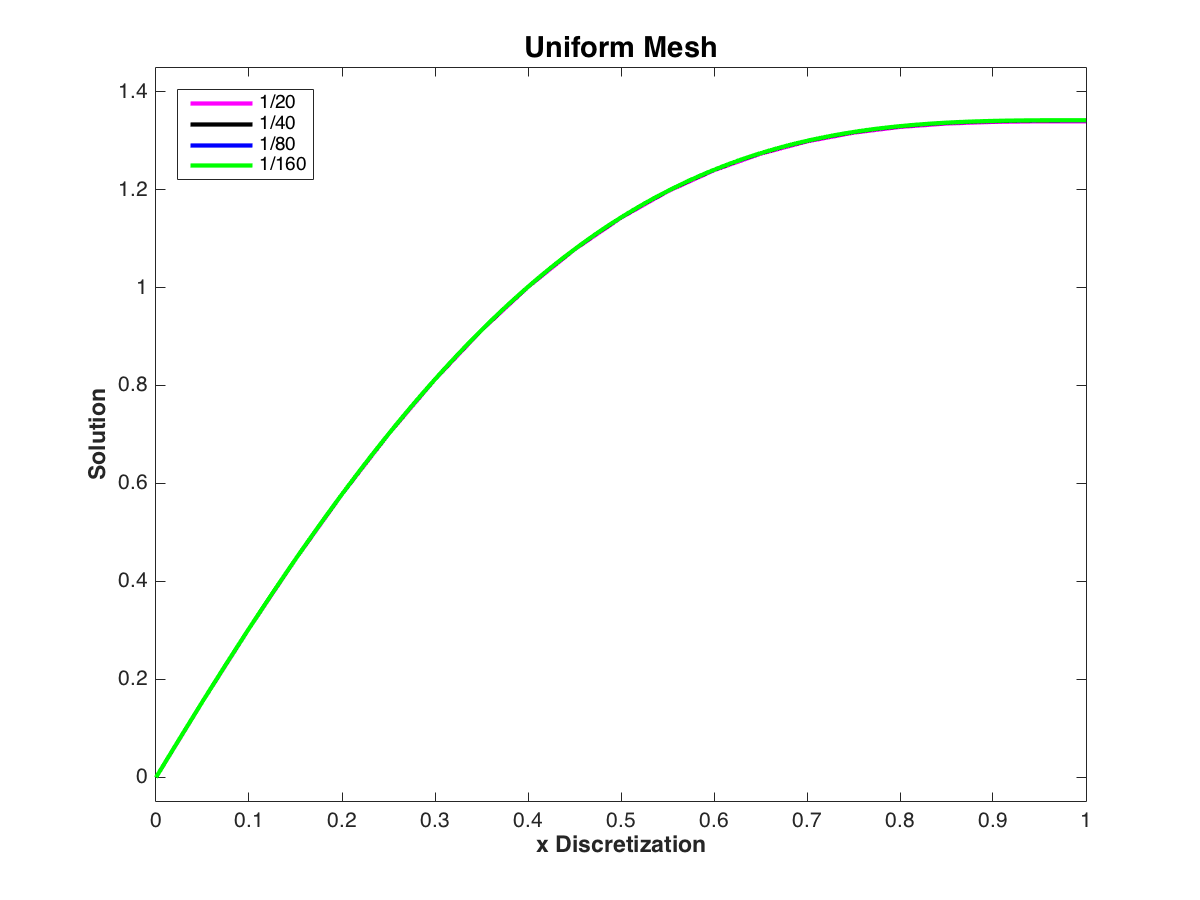
\includegraphics[scale = 0.6]{uniform.png}}}
\centerline{Figure 1. Solution on a Uniform Mesh}

\vspace{2mm}

The next figure shows the solution \textbf{v} on a nonuniform mesh generated by golden ratio subdivision with a uniform base mesh with spacing of $h = \frac{1}{20}$ with different depth refinements.

\vspace{2mm}

\centerline {\frame{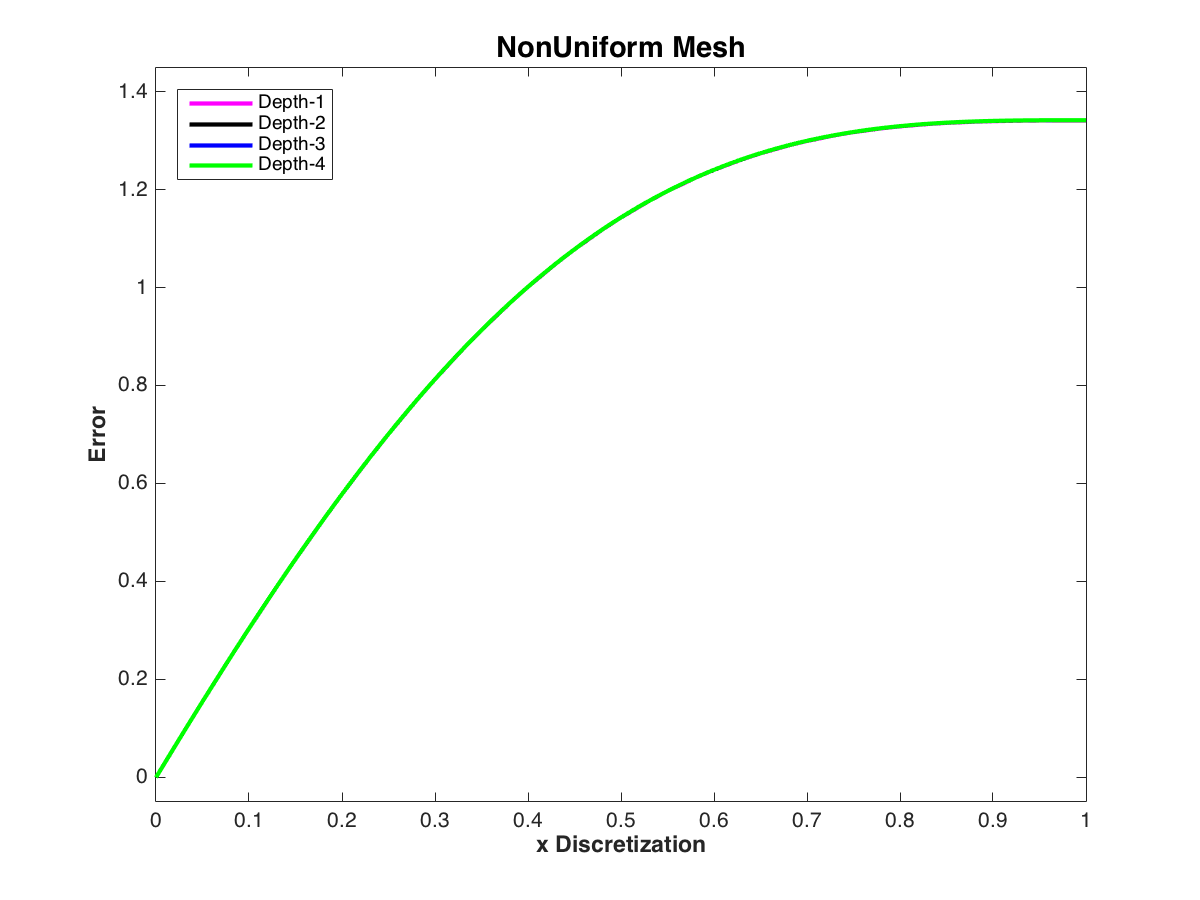
\includegraphics[scale = 0.6]{nonuniform.png}}}
\centerline{Figure 2. Solution on a Nonuniform Mesh}

\vspace{2mm}

We can see that both types of meshes at any depth or step size produce precise and smooth solutions. 

To convince myself that the solution \textbf{v} is second order accurate, I calculated the solution \textbf{v} with a uniform mesh with a step size of $h = \frac{1}{640}$ and took that to be the \emph{true} solution. I compared the coarser meshes at each point to their respective points on the fine mesh. I took the maximum of this error and have shown it in the figures below. I plotted this data on a $\log \log$ plot and to show that it is second order accurate and compared it to step size squared. We can see that these lines clearly have the same slope. It also has the shape we would expect. As the discretization gets larger, so does the error. So the solution \textbf{v} is second order accurate. The same is also true for our nonuniform mesh. I compared the nonuniform mesh error to the uniform step sizes squared as well, even though it doesn't make as much sense, but it does have the same shape and slope which shows that it also confirms that \textbf{v} is second order accurate. 

\vspace{2mm}

\centerline {\frame{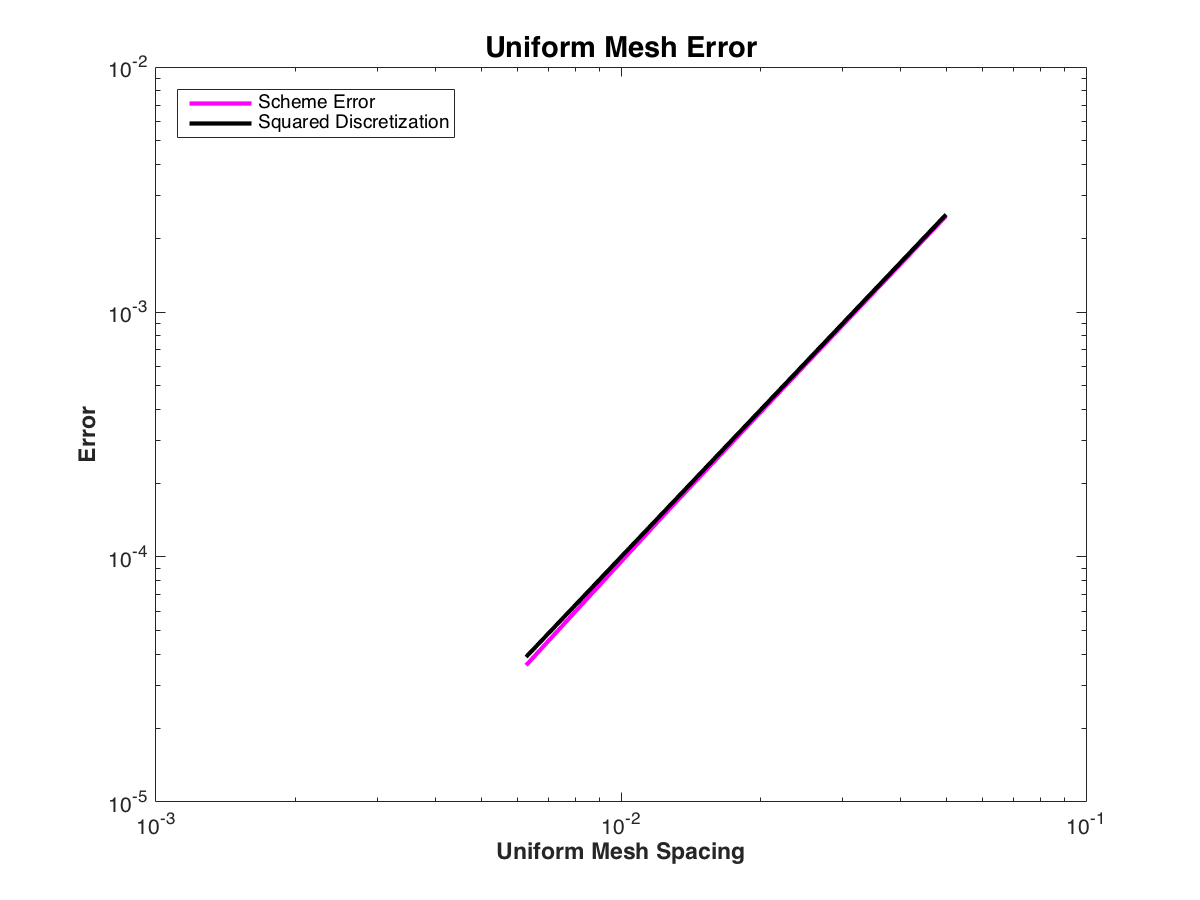
\includegraphics[scale = 0.6]{uniform_error.png}}}
\centerline{Figure 3. Uniform Mesh Error}

\vspace{2mm}

\centerline {\frame{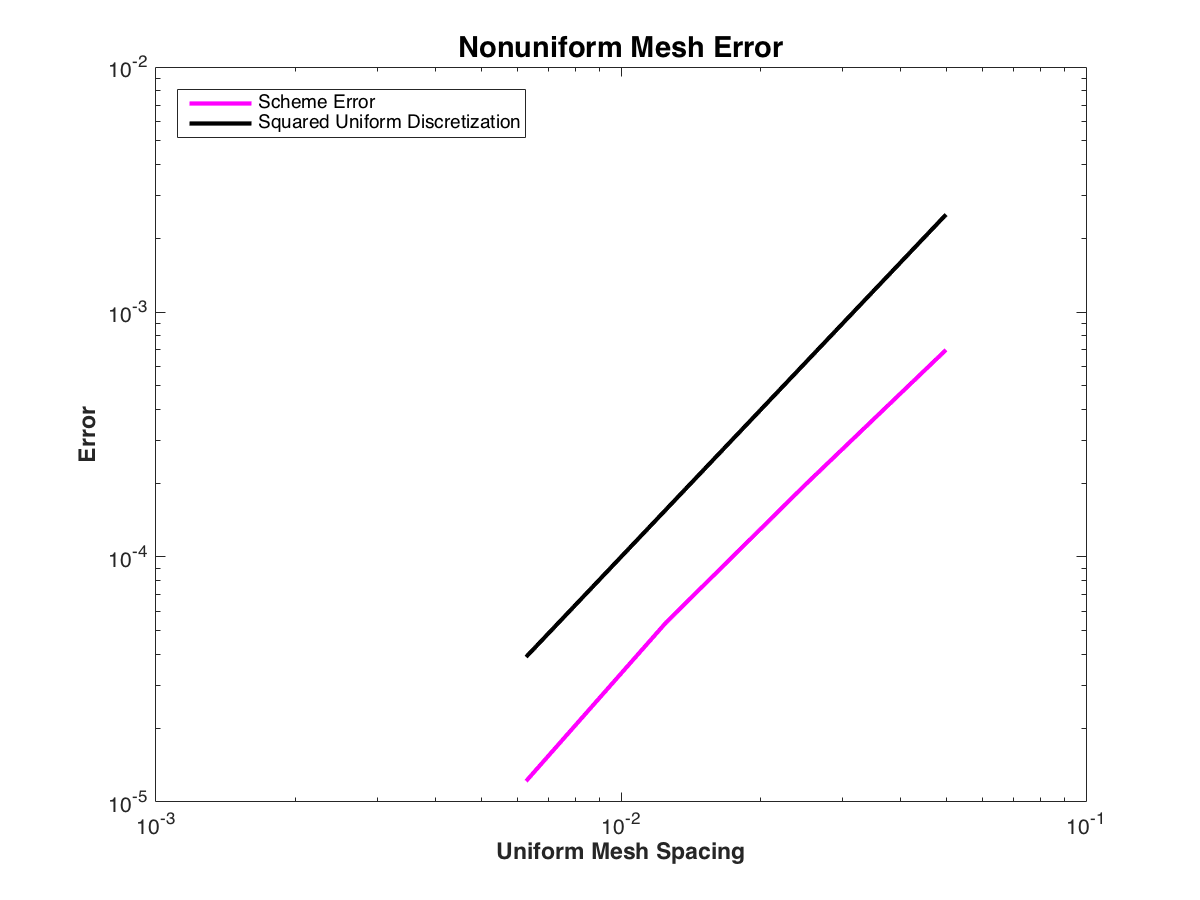
\includegraphics[scale = 0.6]{nonuniform_error.png}}}
\centerline{Figure 4. NonUniform Mesh Error}

To \emph{try} to prove that the solution \textbf{v} is second order accurate, we must recall from problem 1, part a that we discretized the first part of the integral with the midpoint rule which has linear error and equates to the following,
\[
u'_{\text{midpoint}} = \frac{u_{j+1} - u_j}{h_j} + \mathcal{O}(h)
\]

which is squared within the integral and therefore squares the error resulting in a second order accurate solution.

\vspace{2mm}

The MATLAB code for this problem is shown below.

\lstinputlisting{"problem2_main.m"}
\lstinputlisting{"problem2_uniform.m"}
\lstinputlisting{"problem2_nonuniform.m"}

\item 
\subsection{Purpose/Statement of Problem}
For the problem and notation of the previous exercise, define the \textbf{hat function} in one dimension:
\[
\phi_i(x) = \begin{cases}
\frac{x - x_{i-1}}{h_{i-1}}, & x_{i-1} \leq x < x_i,\\
\frac{x_{i+1} -x}{h_i}, & x_i \leq x < x_{i+1},\\
0 & \text{otherwise.}\\
\end{cases}
\]

Derive the Galerkin finite element method for the boundary value ODE. Show that the stiffness matrix $A$ is tridiagonal, symmetric, and positive definite. How does this method relate to the method of the previous exercise?

Write a one-dimensional FEM solver based upon the procedure given in class and repeat the computational experiment above. Comment on your results (and the comparison with the previous problem).

\subsection{Description of Mathematics}

The ODE we are aiming to solve is
\[
-(au')' = q, \quad 0 < x < 1,
\]
\[
u(0) = 0, \quad u'(1) = 0,
\]
where $a(x) > 0$ and $q(x)$ are known, smooth functions. For our computational and mathematical purposes, $a(x) = 1+ e^x$ and $q(x) = \pi^2 \sin(\pi x)$. 

To derive a Galerkin finite element method, we must multiply each side by the \textbf{hat function} and evaluate the integral within the space boundary.
\[
\int_0^1 (au')' \phi_j dx = -\int_0^1 q \phi_j dx
\]
Integration by parts magic gives the following,
\[
au' \phi_j \big |_0^1 - \int_0^1 au' \phi'_j dx = -\int_0^1 q \phi_j dx.
\]
Due to the boundary conditions, the first term equates to zero. If we divide by -1 we get the following,
\[
\int_0^1 au' \phi'_j dx = \int_0^1 q \phi_j dx.
\]
We now define $u = \sum \limits_{i=0}^J \hat u_i \phi_i$ which is the basis decomposition of $u$ with $\phi$. This would result in $u' = \sum \limits_{i=0}^J \hat u_i \phi'_i$. Due to our boundary conditions the limits must be changed resulting in
\[
u = \sum \limits_{i=1}^{J-1} \hat u_i \phi_i, \quad u' = \sum \limits_{i=1}^{J-1} \hat u_i \phi'_i.
\]
We plug this into our above equation,
\[
\int_0^1 \left(\sum \limits_{i = 1}^{J-1} a \hat u_i \phi'_i \right)\phi'_j dx = \int_0^1 q \phi_j dx.
\]
Since both the sum and the integral are finite, they can be switched.
\[
\sum \limits_{i = 1}^{J-1} \left(\int_0^1 a \phi'_i \phi'_j dx\right) \hat u_i = \int_0^1 q \phi_j dx.
\]
We can see that we now have a system of equations to solve for our solution $\hat u_i$. Our stiffness matrix will be the matrix with rows $\left(\int_0^1 a \phi'_i \phi'_j dx\right)$. Calculating both the stiffness matrix and the right hand side is hefty so we will do one at a time. Let's start with the right hand side.
\[
\int_0^1 q \phi_j dx = \int_0^1 \pi^2 \sin(\pi x) \phi_j dx = \int_ {x_{j-1}}^{x_{j+1}} \pi^2 \sin(\pi x) \phi_j dx
\]
We break this integral up because of the \textbf{hat function}.
\[
=\int_ {x_{j-1}}^{x_{j}} \pi^2 \sin(\pi x) \frac{(x - x_{j-1})}{h_{j-1}} dx + \int_ {x_{j}}^{x_{j+1}} \pi^2 \sin(\pi x)\frac{(x_{j+1} - x)}{h_j}dx
\]
By integration by parts and simplification,
\[
\int_0^1 q \phi_j dx = \frac{1}{h_{j-1}} (\sin(\pi x_j) - \sin(\pi x_{j-1})) + \frac{1}{h_j} (\sin(\pi x_j) - \sin(\pi x_{j+1})).
\]
Now let's move on to the stiffness matrix. To get our coefficient terms for each row, there are three cases that we must consider because of the \textbf{hat function}.

\begin{enumerate}

\item \textbf{Case 1:} $j = i-1$
\[
\int_0^1 a \phi'_i \phi'_{i-1} dx = \int_{x_{i-1}}^{x_i} (1+e^x) \left( \frac{1}{h_{j-1}} \right) \left( -\frac{1}{h_{j-1}} \right)dx = -\frac{1}{h_{j-1}^2}(h_{j-1} + e^{x_i} - e^{x_{i-1}})
\]

\item \textbf{Case 2:} $j =1$
\[
\int_0^1 a (\phi'_i)^2 dx = \int_{x_{i-1}}^{x_{i+1}} a (\phi'_i)^2 dx = \int_{x_{i-1}}^{x_i}a (\phi'_i)^2 dx + \int_{x_{i}}^{x_{i+1}} a (\phi'_i)^2 dx
\]

\[
= \int_{x_{i-1}}^{x_i} (1 + e^x) \left( \frac{1}{h_{j-1}} \right)^2 dx + \int_{x_{i}}^{x_{i+1}} (1 + e^x) \left( \frac{1}{h_{j}}\right)^2 
\]

\[
= \frac{1}{h_{j-1}^2}(h_{j-1} + e^{x_i} - e^{x_{i-1}}) + \frac{1}{h_{j}^2}(h_{j} + e^{x_{i+1}} - e^{x_{i}})
\]

\item \textbf{Case 3:} $j = i+1$
\[
\int_0^1 a \phi'_i \phi'_{i+1} dx = \int_{x_{i}}^{x_{i+1}} (1+e^x) \left( \frac{1}{h_{j}} \right) \left( -\frac{1}{h_{j}} \right)dx = -\frac{1}{h_{j}^2}(h_{j} + e^{x_{i+1}} - e^{x_{i}})
\]

\end{enumerate}

\vspace{2mm}

We can see that the stiffness matrix is tridiagonal because it only has three terms in each row centered around the diagonal term. 

We can show that the matrix is symmetric by comparing locations at $(i,i+1)$ and $(i+1,i)$.
\[
S_{(i,i+1)} = -\frac{1}{h_i^2} (h_i + e^{x_{i+1}} - e^{x_i})
\]
Let $j = i+1$ so that $S_{(i,i+1)} = S_{(j,j-1)}$.
\[
S_{(j,j-1)} = -\frac{1}{h_{j-1}^2}(h_{j-1} + e^{x_j} - e^{x_{j-1}})
\]
Putting this back into terms of $i$,
\[
S_{(i,i+1)} = -\frac{1}{h_i^2} (h_i + e^{x_{i+1}} - e^{x_i}).
\]
So the stiffness matrix is symmetric.

To test if the stiffness matrix is positive definite, we will use the following theorem. A symmetric matrix is positive definite if each diagonal entry is equal to the sum of the absolute values of all other entries in the row/column in which it appears with the exception of at least one row where it is greater. This is true for the stiffness matrix due to the boundary conditions which makes the first entry in the first row 1 followed by zeros. We can also see that the rest of the rows are equal.

\subsection{Description of Algorithms}

In my implementation of an FEM solver, I used essentially the same algorithm as the previous problem, but changed coefficients and my evaluation of the right hand side. First, I calculated the solution \textbf{v} with a uniform mesh with a step size of $h = \frac{1}{640}$ and took that to be the \emph{true} solution. I then calculated the solution \textbf{v} at each mesh refinement. I compared the coarser meshes at each point to their corresponding points on the fine mesh. I also did this for the nonuniform mesh, but took a depth of 5 to be the \emph{true} solution.

To compute the uniform solutions and nonuniform solutions, I wrote two separate methods to keep things simple. In both methods, I set the stiffness matrix to have the first and last row to satisfy the boundary conditions. I then set each of the tridiagonal entries to their respective coefficients outlined in the Mathematics section. The nonuniform section will have a specification of the corresponding $h$ values. While I am setting up the stiffness matrix, I am also calculating the corresponding right hand side values. I then solve using both the stiffness matrix and the right hand side. 
\[
x = A^{-1} b
\]

To compute the nonuniform meshes I calculated the "midpoints" using a ratio of $\phi:1$, where $\phi$ is the golden ratio. This resulted in the following equation for the midpoints:
\[
x_{mid} = \frac{\phi x_{i+1} + x_i}{1+\phi}.
\]
I began with a base mesh of $h = \frac{1}{20}$. Then I made a new array of the $x_{mid}$'s, concatenated this to the base mesh and sorted it. I do this again on the concatenated, sorted array for another level of depth.

\subsection{Demonstration of the Correctness of Implementation}

Since this problem was the same computational experiment as the previous problem, I compared their solution results and saw that they were the same.

\subsection{Results/Analysis of Results}

The following figure shows the solution \textbf{v} on a uniform mesh at different mesh refinements solved using a 1D FEM solver.

\vspace{2mm}

\centerline {\frame{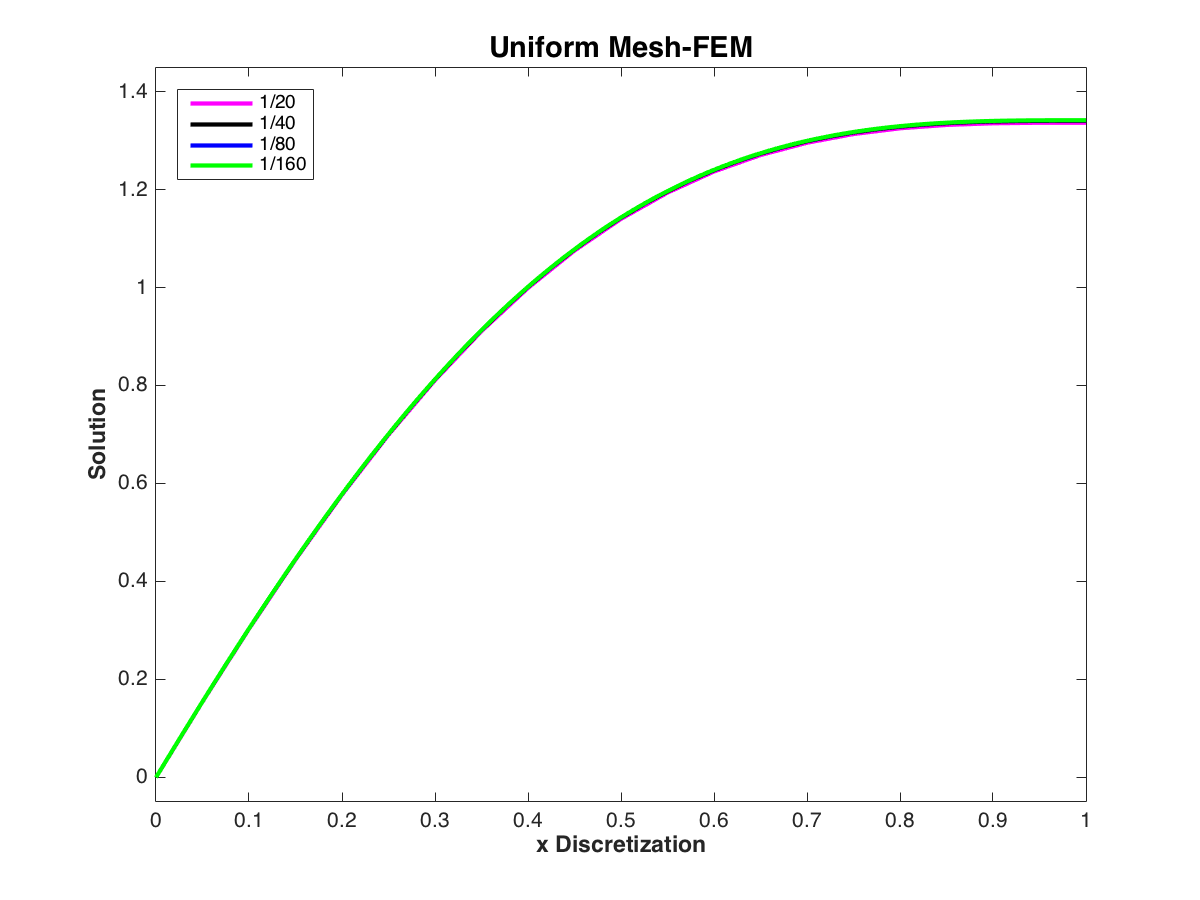
\includegraphics[scale = 0.6]{uniform_FEM.png}}}
\centerline{Figure 5. Solution on a Uniform Mesh with FEM}

\vspace{2mm}

We can see that the functions are smooth and very precise throughout the different mesh refinements. This shape is what we expected to see. 

The next figure shows the solution \textbf{v} on a nonuniform mesh generated by golden ratio subdivision with a uniform base mesh with spacing of $h = \frac{1}{20}$ with different depth refinements solved using a 1D FEM solver.

\vspace{2mm}

\centerline {\frame{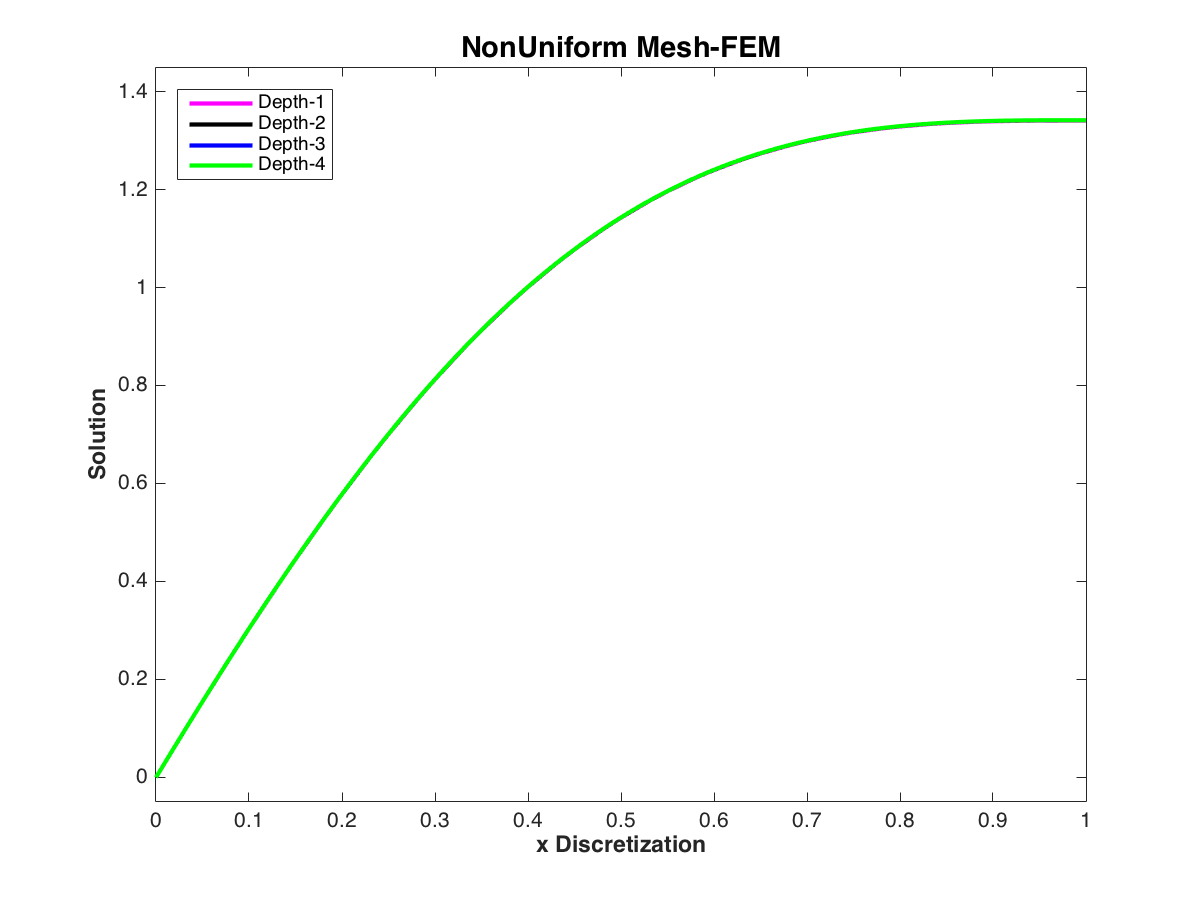
\includegraphics[scale = 0.6]{nonuniform_FEM.png}}}
\centerline{Figure 6. Solution on a Nonuniform Mesh with FEM}

\vspace{2mm}

We can see, again, that the functions are smooth and very precise throughout the different depths. This shape is what we expected to see. The Nonuniform mesh appears to be more precise than the uniform mesh through out the different refinements.

To compare error, like in the previous problem, I took the max of the error for each mesh refinement and have shown it in the figures below. I plotted this data on a $\log \log$ plot and to show that it is second order accurate, I compared it to step size squared. We can see that these lines have the same slope. It also has the shape we would expect. As the discretization gets larger, so does the error. So the solution \textbf{v} is second order accurate. The same is also true for our nonuniform mesh. I compared the nonuniform mesh error to the uniform step sizes squared as well, even though it doesn't make as much sense, but it does have a similar shape and slope. It appears that the nonuniform mesh is somewhere inbetween first and second order accurate.

\vspace{2mm}

\centerline {\frame{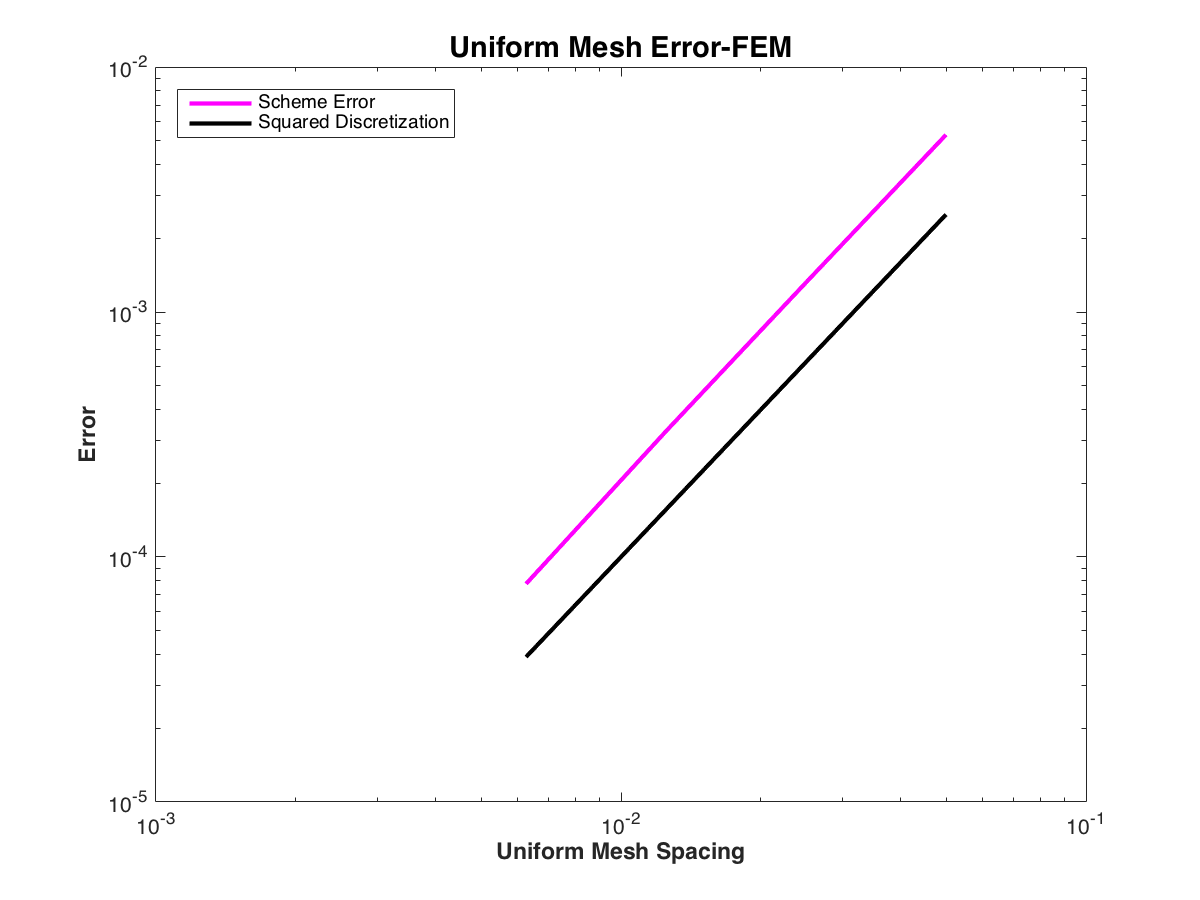
\includegraphics[scale = 0.6]{uniform_error_FEM.png}}}
\centerline{Figure 7. Uniform Mesh Error with FEM}

\vspace{2mm}

\centerline {\frame{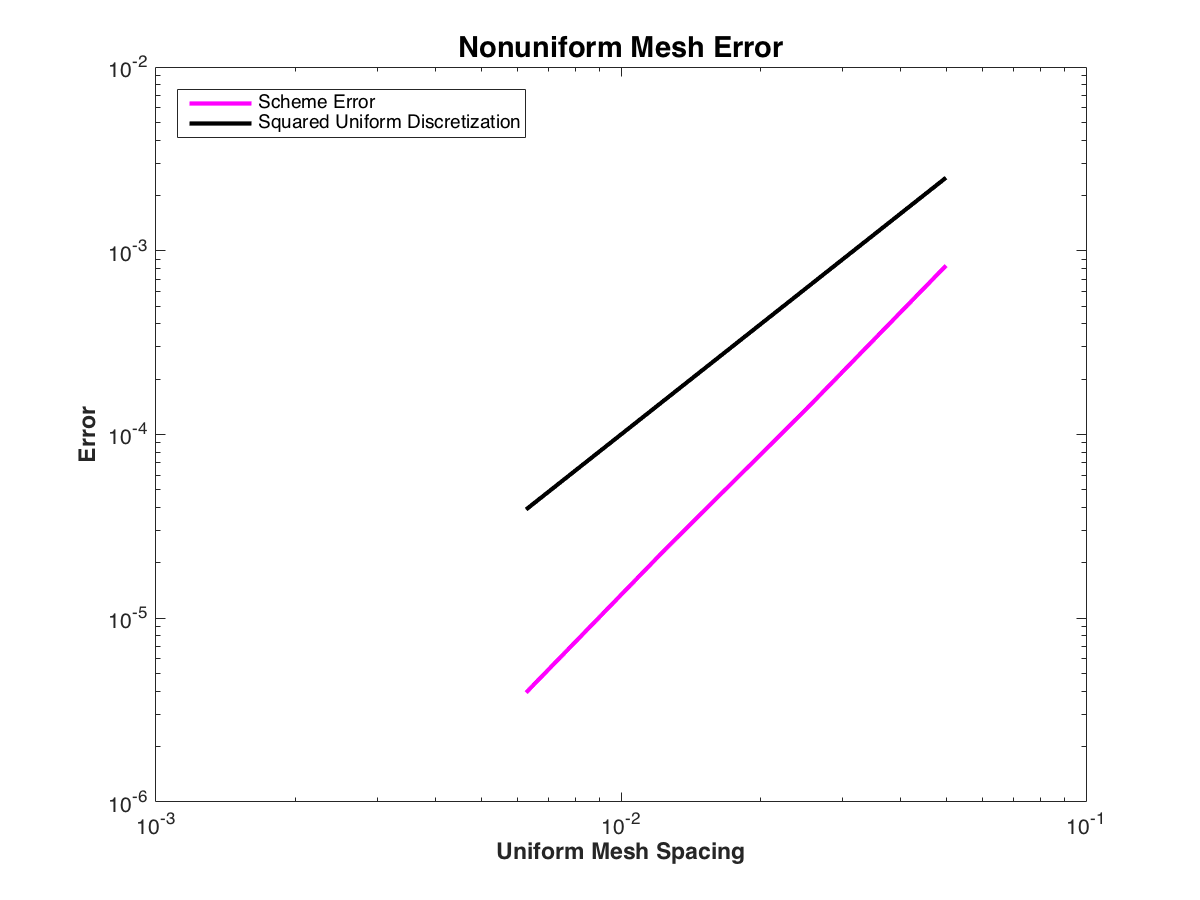
\includegraphics[scale = 0.6]{nonuniform_error_FEM.png}}}
\centerline{Figure 8. NonUniform Mesh Error with FEM}

\subsection{Summary and Conclusions}

Using a 1D FEM solver did not change the shape or size of our solution, but there were changes in error. There was actually less error using an FEM solver with a uniform mesh (in comparison to the previous problem), but it was still second order accurate. Although things did get a bit wonky with the nonuniform mesh being between first and second order accurate using an FEM solver.

\vspace{2mm}

The MATLAB code for this problem is shown below.

\lstinputlisting{"problem3_main.m"}
\lstinputlisting{"problem3_uniform.m"}
\lstinputlisting{"problem3_nonuniform.m"}

\end{enumerate}

Row Oriented:

$\epsilon_1 = \phi1/\lambda_{11}$

do $i = 2,n$

\quad do $j = 1, i-1$

\quad \quad \phi_i = \phi_i = \lambda_{ij} \epilon_j

\end{document}